%%%%%%%%%%%%%%%%%%%%%%%%%%%%%%%%%%%%%%%%%%%%%%%%%%%%%%%%%%%%%%%%%%%%%%%%%%
%%%%%%%%%%%%   CAPTER 1   %%%%%%%%%%%%%%%%%%%%%%%%%%%%%%%%%%%%%%%%%%%%%%%%
%%%%%%%%%%%%%%%%%%%%%%%%%%%%%%%%%%%%%%%%%%%%%%%%%%%%%%%%%%%%%%%%%%%%%%%%%%
\chapter{Introduction}
\label{chap:introduction}

Stereo vision is a method of extracting 3D information from 2D images taken from different viewpoints using multiple cameras \cite{young_ki_baik_fast_2006}. It is similar to the biological process of Stereopsis. There are many types of Stereo vision system depending upon the number of cameras and usage of illumination. The type of Stereo vision dealt with in this thesis is the passive binocular Stereo vision which involves laterally shifted images taken from two cameras. It can be seen as illustrated in the forthcoming chapter that in such a system, closer an object is to the camera pair higher will the be shift in its position in the image taken by one camera to other. Stereo vision finds its application in 3D reconstruction, autonomous navigation, gaming etc.\\
\\
GPUs are many-core processors capable of very high computation and data throughput. Traditionally GPUs were particularly designed for computer graphics applications and were not easy to program. But subsequently they are evolving into general-purpose parallel processors capable of being programmed in industry standard languages like C. GPGPU stands for General-Purpose computation on Graphics Processing Units \cite{harris_about}. Embedded GPUs (eGPUs) are GPUs with fewer cores compared to traditional GPUs. The GPU cores of an embedded GPU are realised in the same chip as the host CPU of the system. In contrast to traditional GPUs, eGPUs usually share the main memory with the host CPU as shown in the Figure \ref{fig:gpuegpu}. They are devices which support parallel processing in power critical situations. One example of such a situation is on the mobile phone where battery life is a critical parameter. Example of an eGPU is NVIDIA's Tegra processor, which has 192 GPU cores in it.\\

\begin{figure}
\begin{subfigure}{.5\textwidth}
  \centering
  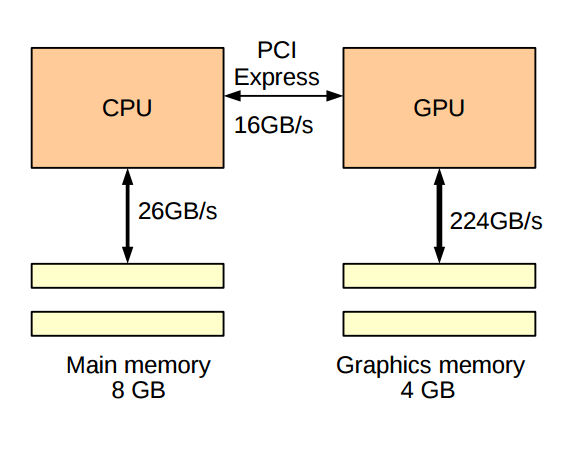
\includegraphics[width=.8\linewidth]{figures/memorygpu}
  \caption{GPU}
  \label{fig:sfig1}
\end{subfigure}%
\begin{subfigure}{.5\textwidth}
  \centering
  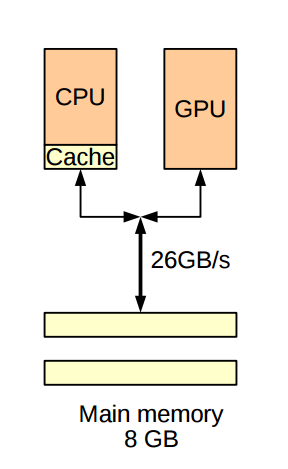
\includegraphics[width=.4\linewidth]{figures/memoryegpu}
  \caption{eGPU}
  \label{fig:sfig2}
\end{subfigure}
\caption{Memory organisation \cite{Collange2015}}
\label{fig:gpuegpu}
\end{figure}

Critical metrics of an eGPU for any application include functionality and its execution time. In the following thesis, a Stereo vision algorithm is chosen as a baseline, optimizations are done on the algorithm, and the metrics of an eGPU from ThinkSilicon called Nema are evaluated.\\

%%%%%%%%%%%%%%%%%%%%%%%%%%%%%%%%%%%%%
%%%%%%%%%%%%%%%%%%%%%%%%%%%%%%%%%%%%%
%%%%%%%%%%%%   SECTION   %%%%%%%%%%%%
%%%%%%%%%%%%%%%%%%%%%%%%%%%%%%%%%%%%%
%%%%%%%%%%%%%%%%%%%%%%%%%%%%%%%%%%%%%
\section{Problem Statement}
\label{sec:intro:probstatement}

Stereo vision is an active field with lot of ongoing research. There are many approaches for disparity map (DM) creation in a passive binocular Stereo vision system. The functional performance of an algorithm is highly dependent on the parameters chosen. Execution time of an algorithm is also a critical factor in a Stero vision application. A study of parameter variations and software optimizations on a Stereo vision algorithm are required for a better understanding of the algorithm. 

Think silicon Ltd. has developed a new version of eGPU called Nema. The GPU has to be tested out for a real world application. A suitable application for the eGPU could be a passive binocular Stereo vision system. An algorithm needs to be chosen for the Stereo vision application. The parameters of the algorithm need to be finalised. Possible software optimizations need to be done to improve the execution time of the algorithm. Further acceleration of the algorithm facilitated by the GPU needs to be measured. Any bottleneck causing reduction in the acceleration of the system needs to be identified and reasoned out.


%%%%%%%%%%%%%%%%%%%%%%%%%%%%%%%%%%%%%
%%%%%%%%%%%%%%%%%%%%%%%%%%%%%%%%%%%%%
%%%%%%%%%%%%   SECTION   %%%%%%%%%%%%
%%%%%%%%%%%%%%%%%%%%%%%%%%%%%%%%%%%%%
%%%%%%%%%%%%%%%%%%%%%%%%%%%%%%%%%%%%%
\section{Contributions}
\label{sec:intro:contrib}

Stereo vision is an active and one of the most heavily investigated areas of computer vision. One of the major applications of Stereo vision system is in autonomous robotics \cite{pinhas_ben-tzvi_embedded_2010}. In many applications under autonomous robotics, like drones, the size and the power consumption of the system plays an important role. eGPU based hardware provide a very good trade-off between the size, power and performance for embedded applications. Hence, investigation of a performance of eGPU running a Stereo vision algorithm serves as an important research topic.
%

In summary, the main contributions of this thesis are:

\begin{itemize}
\item{Algorithm choice and Optimizations}
  \begin{itemize}
    \item Choice of a Stereo vision algorithm and its parameters for the eGPU evaluation.
    \item Software optimizations of the algorithm for faster execution time.
    \item Measurement of functional and run-time performance of various versions of the algorithm in different hardware.
  \end{itemize}
\item {eGPU evaluation}
     \begin{itemize}
    \item Implementation of the algorithm in Nema eGPU.
    \item Report of functional verification and acceleration provided by eGPU
    \item Detecting and reasoning out of bottlenecks.
    \end{itemize}
\end{itemize}
%%%%%%%%%%%%%%%%%%%%%%%%%%%%%%%%%%%%%
%%%%%%%%%%%%%%%%%%%%%%%%%%%%%%%%%%%%%
%%%%%%%%%%%%   SECTION   %%%%%%%%%%%%
%%%%%%%%%%%%%%%%%%%%%%%%%%%%%%%%%%%%%
%%%%%%%%%%%%%%%%%%%%%%%%%%%%%%%%%%%%%
\section{Thesis outline}
\label{sec:intro:outline}

The rest of this thesis is organized as follows:

\begin{compactitem}
  \item Chapter 2 focuses on the background of Stereo vision. The hardware and software components of GPUs in general and Nema in particular are discussed. Kernel and mapping information of the eGPU is provided. Related work in the field are discussed.
  \item Chapter 3 discusses on the Stereo vision algorithm. It also provides information on various optimizations done on the algorithm.
  \item Chapter 4 discusses on the software implementation of the algorithm. Results of parameteric variations and execution time of various optimized versions of the algorithm in different hardware are presented. 
  \item Chapter 5 discusses on the eGPU implementation of the algorithm. The functionality and the execution time of the algorithm on the GPU is discussed. Comments on the eGPU based on the observations are presented.
  \item Chapter 6 provides the conclusion, suggestions for imrprovement. Future work in the lines are discussed.
\end{compactitem}